\documentclass{beamer}
% \includeonlyframes{current}
\setbeamertemplate{navigation symbols}{}

\title{Bayesian nonparametric model for gene expression}
\author{Eric Mittman \\ \vspace{.5cm} Advisor: Jarad Niemi}

%includes
\usepackage{amsmath, bbm, blkarray}
\usepackage{graphicx}
\usepackage{natbib}
% \usepackage{tikz}
% %include tikz
% \usepackage{tikzscale}
% \usetikzlibrary{arrows,decorations.pathmorphing,backgrounds,matrix,positioning,fit,petri, external}
\usepackage{booktabs}
\usepackage{multirow,makecell}
%\tikzexternalize[prefix=tikz/]

%theme
\usetheme{Dresden}
\usefonttheme[onlymath]{serif}

%colors
% Custom colors
\usepackage{xcolor}
\definecolor{gold}{HTML}{F1BE48}
\definecolor{red}{HTML}{C8102E}
\setbeamercolor{upcol}{fg=black,bg=red}
\setbeamercolor{lowcol}{fg=black,bg=gold!40}
\usecolortheme[named=red]{structure}

%macros
\newcommand{\mc}{\mathcal}
\newcommand{\mb}{\mathbb}
\newcommand{\op}{\operatorname}
\newcommand{\ind}{\stackrel{ind}{\sim}}
\newcommand{\iid}{\stackrel{ind}{\sim}}

\AtBeginSection[]{
  \begin{frame}
  \vfill
  \centering
  \begin{beamercolorbox}[sep=8pt,center,shadow=true,rounded=true]{title}
  \usebeamerfont{title}\secname\par%
  \end{beamercolorbox}
  \vfill
  \end{frame}
}

\graphicspath{{../chapter1/figures_tables/}{../chapter2/figures_tables/}{../chapter3/figures_tables/}}

\begin{document}


\frame{\titlepage}

% \begin{frame}
% \frametitle{Table of Contents}
% \tableofcontents
% \end{frame}

%%% Section 0: Data problem
\section[Gene Expr.]{Gene expression profiling}

\begin{frame}%[label=current]
\frametitle{``Gene expression" $=$ Transcript abundance}
{\scriptsize \citep[\textit{Statistical Analysis of Next Generation Sequencing Data}]{datta2014}}
The Central Dogma of Biology says:
\begin{itemize}
\pause\item DNA encodes all biological information
\pause\item Genes (regions of the DNA) encode directions for assembling proteins
\pause\item messenger RNA (mRNA) conveys ``transcripts" of these directions to the ribosomes where they are assembled 
\end{itemize}
\pause Transcript abundance is proxy for gene expression.
\end{frame}

\begin{frame}%[label=current]
\frametitle{Gene expression profiling - RNA-seq}
\pause RNA-seq is:
\vspace{.5cm}
\begin{itemize}
\pause \item "whole transcriptome shotgun sequencing"
\pause \item simultaneously measurement of transcript abundance of thousands of genes
\pause \item sequencing is high resolution
\end{itemize}

\vspace{.5cm}
Stages of RNA-seq data production:
\vspace{.5cm}
\begin{itemize}
\pause \item isolate mRNA
\pause \item fragmentation
\pause \item amplification
\pause \item sequencing/matching fragments back to genes/features (counts)
\end{itemize}
\end{frame}

\begin{frame}%[label=current]
\frametitle{RNA-seq data}

% latex table generated in R 3.4.2 by xtable 1.8-2 package
% Fri Dec 01 15:02:44 2017
\begin{table}[ht]
\scalebox{.7}{
\centering
\begin{tabular}{crrrrrr}
  \toprule
& \multicolumn{3}{c}{Alcoholic Liver} & \multicolumn{3}{c}{Normal Liver} \\
  \midrule
& Sample 1 & Sample 2 & Sample 3 & Sample 1 & Sample 2 & Sample 3 \\ 
  \midrule
Gene 1 &    5 & 0 & 3 & 3 & 0 & 4 \\ 
Gene 2 &  3637 & 2730 & 2797 & 2003 & 1734 & 2598 \\ 
Gene 3  & 40 & 45 & 59 & 6 & 4 & 6 \\ 
Gene 4 &  69 & 67 & 64 & 14 & 5 & 10 \\ 
\vdots & & & & & &\\
\midrule
raw library size  &11569434 & 10079799 & 9028465 & 10028258 & 9010306 & 10283594 \\ 
   \bottomrule
\end{tabular}
}
\end{table}
\begin{itemize}
\pause \item Overdispersed counts (contain zeros)
\pause \item Small samples are typical
\pause \item Our approach: fit a hierarchical model to borrow information across genes
\end{itemize}
\end{frame}

\begin{frame}%[label=current]
\frametitle{Motivating example - Heterosis}
\begin{columns}
\begin{column}{.3\textwidth}
\begin{table}
\begin{tabular}{c}
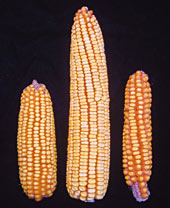
\includegraphics[height=.35\textheight]{BFMears}\\
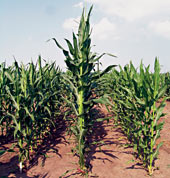
\includegraphics[height=.35\textheight]{BFMfield}
\end{tabular}
{\scriptsize \url{https://archive.news.iastate.edu/news/2006/may/vigor.shtml}}
\end{table}
\end{column}

\begin{column}{.7\textwidth}
\scalebox{.9}{
  \begin{beamerboxesrounded}[upper=upcol,lower=lowcol,shadow=true]{Heterosis}\begin{itemize}
      \pause\item Heterosis $=$ ``Hybrid vigor"
      \pause \item Superior traits in hybrid offpring compared with inbred parents
      \pause \item Want to identify genetic links
    \end{itemize}
    \vspace{.5cm}
    \pause average hybrid expression more extreme than parental expression
    \begin{itemize}
    \pause \item high-parent heterosis (HPH):\\low parent $<$ high parent $<$ hybrid
    \pause \item low-parent heterosis (LPH):\\ hybrid $<$ low parent $<$ high parent
    \end{itemize}
  \end{beamerboxesrounded}
  \onslide<1->
}
\end{column}
\end{columns}
\end{frame}


\begin{frame}%[label=current]
\frametitle{Data from \citet{paschold}}
Produced 16 RNA samples from primary roots of 3.5 day old maize seedlings (each produced from 10 individuals) with aim to identify genes responsible for hybrid vigor (heterosis).
\vspace{.5cm}
\pause\begin{beamerboxesrounded}[upper=upcol,lower=lowcol,shadow=true]{}
\begin{itemize}
\item 2 recombinant inbred lines (homozygous): B73, Mo17
\item 2 reciprocal hybrid crosses: B73$\times$Mo17, Mo17$\times$B73
\item 4 replicates of each variety
\item sequencing done on 2 flow cells, genotypes balanced across flow cells
\end{itemize}
\end{beamerboxesrounded}
\end{frame}

\begin{frame}%[label=current]
\frametitle{Gene-specific parameters}
\begin{beamerboxesrounded}[upper=upcol,lower=lowcol,shadow=true]{model matrix} \scalebox{.6}{
  \begin{equation*}
  \begin{blockarray}{rrrrrr}
    \mbox{Sample} & \mbox{intercept} & \mbox{parental HD} & \mbox{hybrid} & \mbox{hybrid HD} & \mbox{flow cell}\\
    \begin{block}{r(rrrrr)}
    \mbox{B73}_1  & 1 &  1 & 0 & 0 & 0\\
    \mbox{B73}_2  & 1 &  1 & 0 & 0 & 0\\
    \mbox{B73}_3  & 1 &  1 & 0 & 0 & 1\\
    \mbox{B73}_4  & 1 &  1 & 0 & 0 & 1\\
    \mbox{B73}\times\mbox{Mo17}_1  & 1 &  0 & 1 & 1 & 0\\
    \mbox{B73}\times\mbox{Mo17}_2  & 1 &  0 & 1 & 1 & 0\\
    \mbox{B73}\times\mbox{Mo17}_3  & 1 &  0 & 1 & 1 & 1\\
    \mbox{B73}\times\mbox{Mo17}_4  & 1 &  0 & 1 & 1 & 1\\
    \mbox{Mo17}\times\mbox{B73}_1  & 1 &  0 & 1 & -1 & 0\\
    \mbox{Mo17}\times\mbox{B73}_2  & 1 &  0 & 1 & -1 & 0\\
    \mbox{Mo17}\times\mbox{B73}_3  & 1 &  0 & 1 & -1 & 1\\
    \mbox{Mo17}\times\mbox{B73}_4  & 1 &  0 & 1 & -1 & 1\\
    \mbox{Mo17}_1 & 1 & -1 & 0 & 0 & 0\\
    \mbox{Mo17}_2 & 1 & -1 & 0 & 0 & 0\\
    \mbox{Mo17}_3 & 1 & -1 & 0 & 0 & 1\\
    \mbox{Mo17}_4 & 1 & -1 & 0 & 0 & 1
    \end{block}
  \end{blockarray}
  \end{equation*}
}
\end{beamerboxesrounded}
\end{frame}

\begin{frame}%[label=current]
\frametitle{Gene-specific parameter estimates}
{\centering
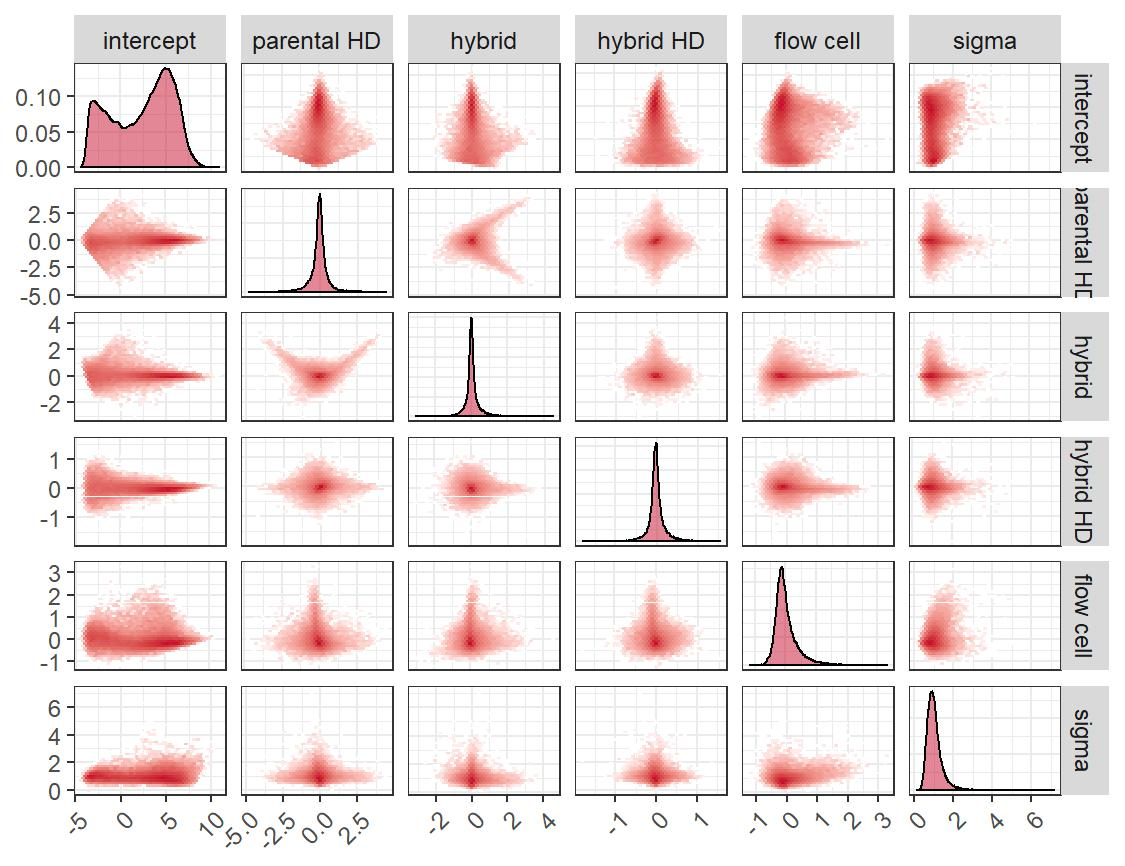
\includegraphics[width=.8\textwidth]{pairs1}\\
}
\end{frame}

%%%%%%%%%%%%%%
\section[DP intro]{The Dirichlet process}

\begin{frame}%[label=current]
\scalebox{.8}{
  \begin{beamerboxesrounded}[upper=upcol,lower=lowcol,shadow=true]{Stick-breaking representation}
    $\mathcal{P}$ = a random probability measure$\\
    \pause $\mathcal{P} \sim \op{DP}(\alpha Q) \implies$
    \begin{itemize}
      \pause \item $\mathcal{P} \stackrel{d}{=} \sum_{k=1}^\infty \pi_k \delta_{\tilde{\mu}_k},\;$ where $\delta_{\cdot}$ is the Dirac delta function, \pause
      \item $\tilde{\mu}_k \ind Q$ \pause and
      \item $\frac{\pi_k}{1-\sum_{\ell<k} \pi_\ell}=\nu_k \ind \op{Be}(1,\alpha)$
    \end{itemize}
    \vspace{.5cm}
    \pause Finite approximation: choose large $K$, set $\nu_K=1$, implying, for $\ell>K$, $\pi_\ell=0$.\\
    \onslide<1->
    \citep{sethuraman,ishwaran2000}
  \end{beamerboxesrounded}
}
\end{frame}

\begin{frame}%[label=current]
\frametitle{DP as infinite mixture ($Q=\op{N}(0,1)$)}
\scalebox{.7}{
  \begin{table}
  \centering
  \begin{tabular}{crl}
  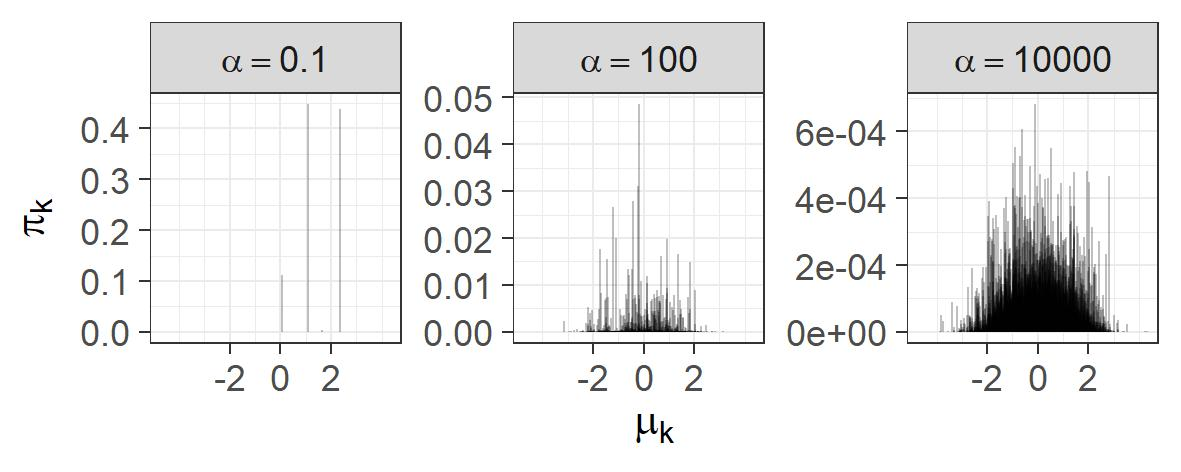
\includegraphics[height=.4\textwidth]{dp1}& \multirowcell{2}{\large $Q=$\\$\alpha=$} & \multirowcell{2}{\large ``prior guess" \\ ``prior sample size"}\\
  \pause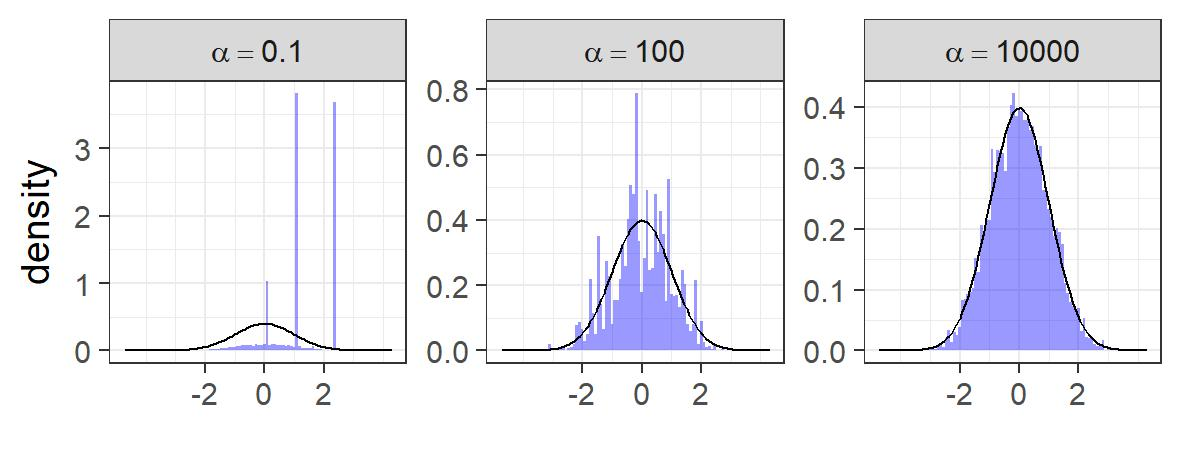
\includegraphics[height=.4\textwidth]{dp2}&&\\
  \end{tabular}
  \end{table}
  \onslide<1->
}
\end{frame}

\begin{frame}%[label=current]
\frametitle{Example: DP as random effects model}
{\small Suppose we observe $y_{gn};\; g=1,\ldots,200,\; n=1,\ldots,3$ where\\
    \pause\[ y_{gn} \sim \op{N}(\mu_g,\sigma^2),\mbox{ with }\{\mu_g\},\sigma_g\mbox{ unknown.}\]
 \pause $\bar{y}_{g\cdot}$ (unbiased for $\mu_g$) are shown below:\\
 {\centering 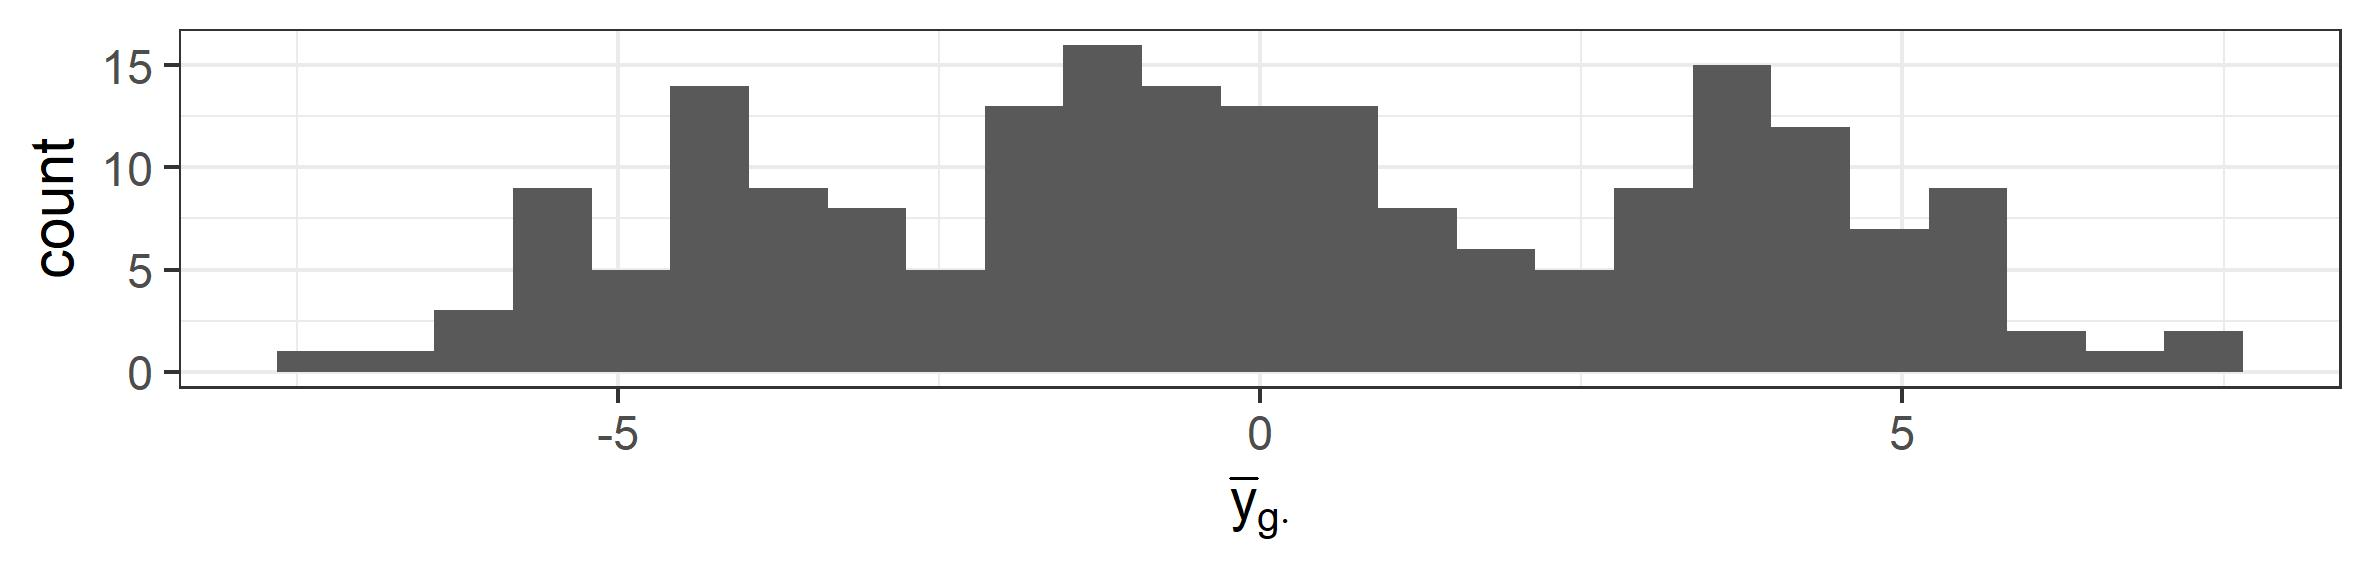
\includegraphics[width=.9\textwidth]{samplemeans_ie}}\\

\pause $\mu_g$ were in fact simulated from $1/3\op{N}(-4,1^2) + 1/3\op{N}(0,1^2) + 1/3\op{N}(4,1^2)$.
}
\end{frame}

\begin{frame}%[label=current]
\frametitle{Example: DP as random effects model}
{\footnotesize
 {\centering 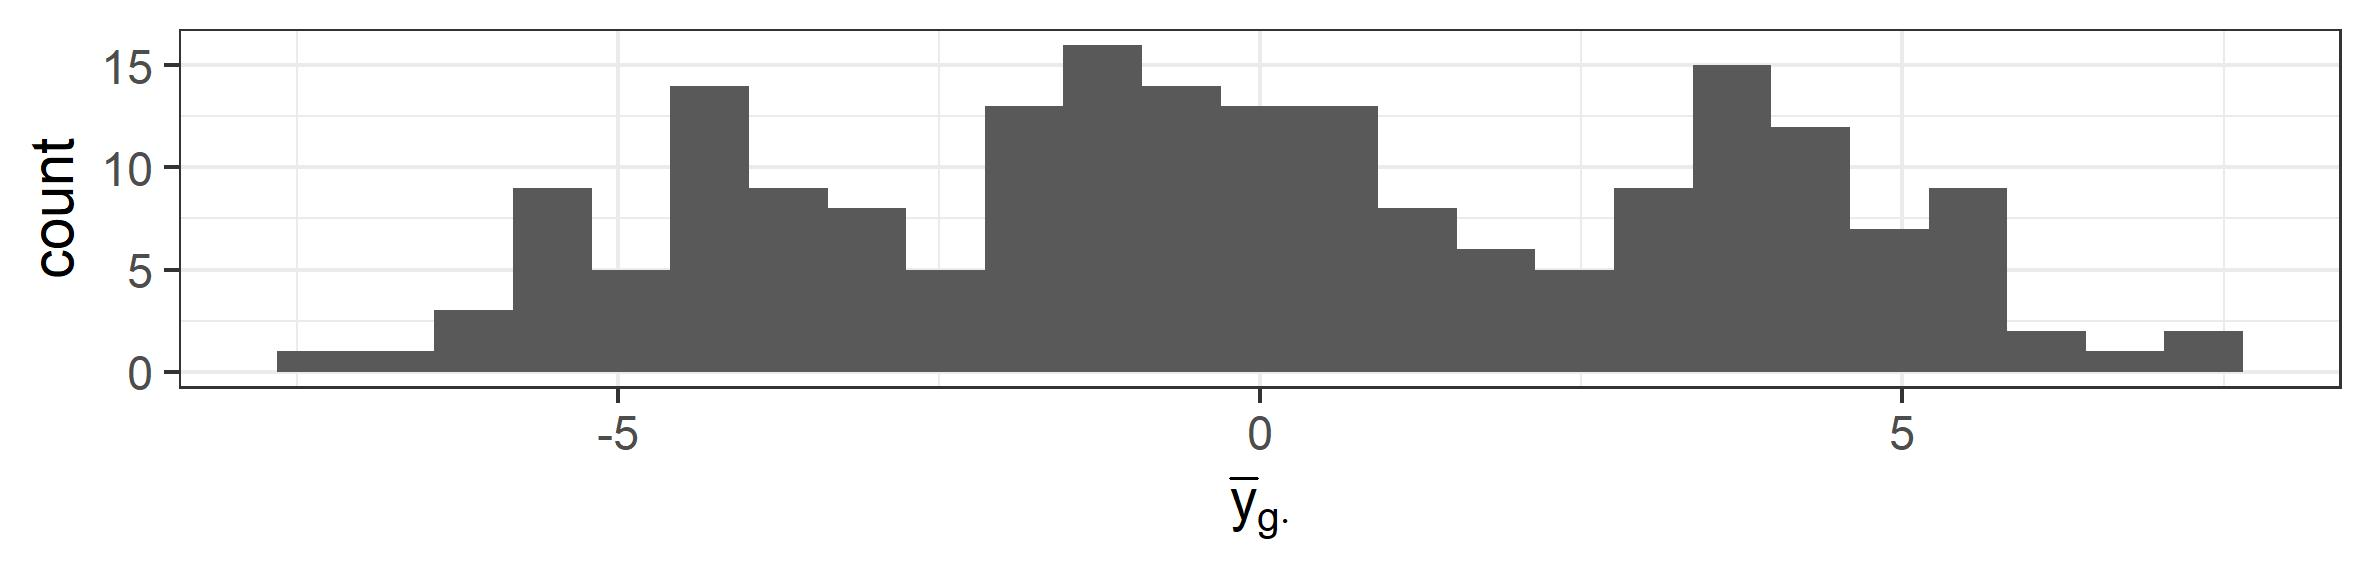
\includegraphics[width=.9\textwidth]{samplemeans_ie}}
 Consider these models for $\mu_g$:
 \begin{enumerate}
  \pause \item (Normal) $\mu_g \ind N(\eta, \tau^2)$\\
     with prior distributions $\eta \sim N(0, 5^2)$, $\tau^2 \sim \op{IG}(0.5,0.5)$
  \pause \item (Correct) $\mu_g \ind \pi_1 \op{N}(\eta_1, \tau^2)+\pi_2 \op{N}(\eta_2, \tau^2_2) + \pi_3 \op{N}(\eta_3,\tau^2)$ with prior distributions \\ $\eta_j \ind N(0,5^2)$, $\tau^2 \sim $\op{IG}(0.5,0.5)$ and $\pi \sim \op{Dir}(1,1,1)$, subject to $\eta_1<\eta_2<\eta_3$.
   \pause \item (DP) $\mu_g \ind \mathcal{P},\; P \sim DP(\alpha Q)$ with $Q \stackrel{d}{=}\op{N}(0,5^2)$, and prior $\alpha \sim \op{Ga}(3,3/14.2)$
     \end{enumerate}
}
\end{frame}

\begin{frame}%[label=current]
\frametitle{Posterior CI width and coverage}
{\centering
  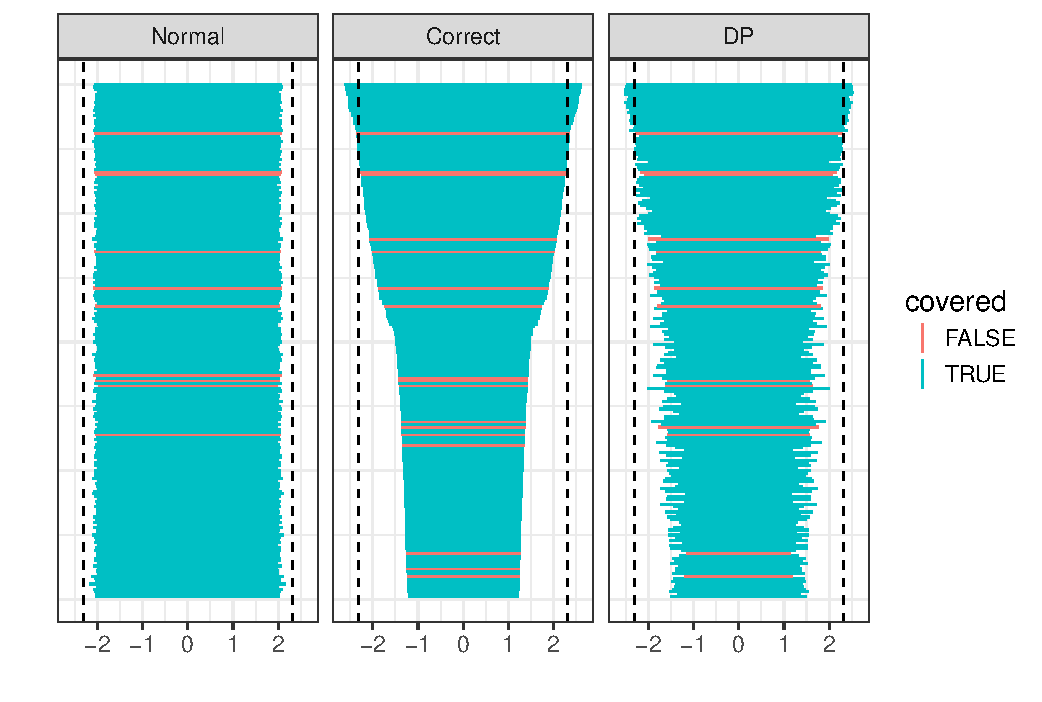
\includegraphics[height=.95\textheight]{cis_12_5}
}
\end{frame}

\begin{frame}%[label=current]
\frametitle{Example - posterior predictive density}
Can the posterior uncover the true data generating mechanism?\\
\pause Pointwise intervals for predictive density:
\begin{enumerate}
\pause \item (Normal) $p(\mu_{new}|\eta,\tau^2)$ w.r.t. $p(\eta,\tau^2|y)$
\pause \item (Correct) $p(\mu_{new}|\eta_1,\eta_2,\eta_3,\tau^2)$ w.r.t. $p(\eta_1,\eta_2,\eta_3,\tau^2|y)$
\pause \item (DP) Posterior draws of $\mathcal{P}$ do not have a density w.r.t. Lebesgue measure \pause ---  instead we use kernel density estimator $\sum_{k=1}^K \pi_k K_h(\mu_{new}-\tilde{\mu}_k)$ w.r.t. $p(\tilde{\mu},\pi|y)$ with a small bandwidth (0.2).
\end{enumerate}
\end{frame}

\begin{frame}%[label=current]
\frametitle{Example - posterior predictive density}
\centering
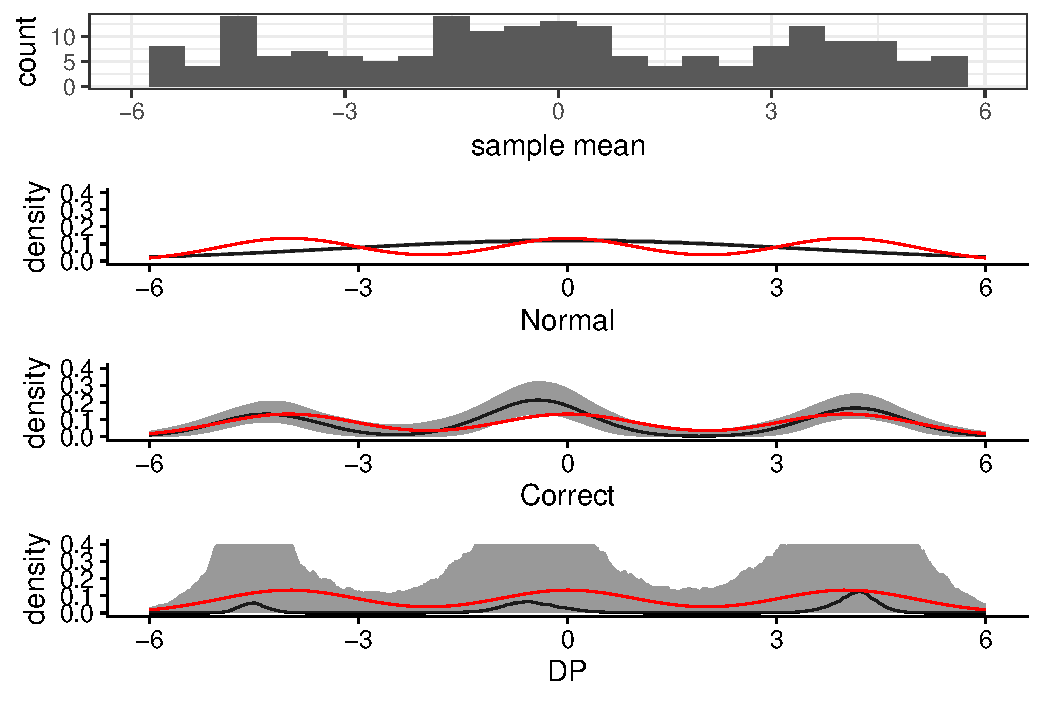
\includegraphics[height=.92\textheight]{predictive_12_5}
\end{frame}

\begin{frame}%[label=current]
\frametitle{Gene-specific parameter estimates}
{\centering
  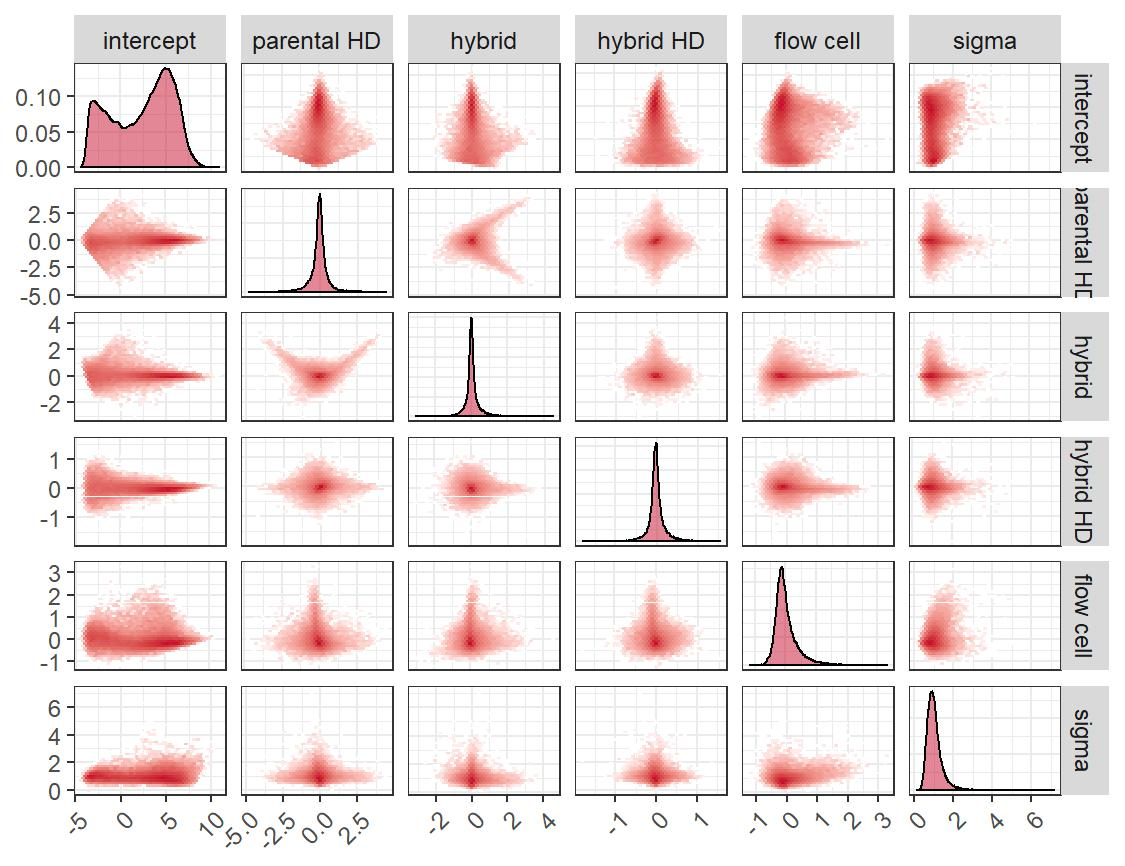
\includegraphics[width=.8\textwidth]{pairs1} \\
}
\end{frame}

%%%%%%%%%%%%%
\section[BNP model]{BNP model for gene expression}

\begin{frame}[label=current]
\frametitle{BNP model}
\scalebox{.8}{
  \begin{beamerboxesrounded}[upper=upcol,lower=lowcol,shadow=true]{Definitions}
  \[y_{g} \ind \op{N}(X\beta_g, \sigma_g^2W_g^{-1}),\]
  \[(\beta_g^\top,\sigma_g^2) \ind \mathcal{P},\]
  \[\mathcal{P} \sim \op{DP}(\alpha Q),\]
  \pause where
  \begin{itemize}
  \item$y_{g}$ is $N$-vector of log counts per million (log-cpm) for gene $g$
  \pause \item $X$ is the model matrix, with rank $p$,
  \pause \item $W_g^{-1}$ is a known diagonal matrix of precision weights,
  \pause \item $Q$ is product measure $\op{N}(m,C)\times\op{IG}(a_\sigma,b_\sigma).$
  \end{itemize}
  \end{beamerboxesrounded}
  \onslide<1->
}
\end{frame}

\begin{frame}[label=current]
\frametitle{Dirichlet process (DP)}
\scalebox{.8}{
  \begin{beamerboxesrounded}[upper=upcol,lower=lowcol,shadow=true]{Stick-breaking representation \citep{sethuraman}:}
    $\mathcal{P} \sim \op{DP}(\alpha Q)$ \pause $\implies$
    \begin{itemize}
      \item $\mathcal{P} \stackrel{d}{=} \sum_{k=1}^\infty \pi_k \delta_{(\tilde{\beta}_k^\top,\tilde{\sigma}^2_k)},\quad$ where $\delta_{}$ is the Dirac delta function \pause with
      \item $(\tilde{\beta}_k^\top,\tilde{\sigma}^2_k) \ind Q$ \pause and
      \item $\nu_k = \frac{\pi_k}{1-\sum_{\ell<k} \pi_\ell} \ind \op{Be}(1,\alpha)$, $k<K-1$.
      \item $\nu_K = 1 \implies \pi_\ell =0$ for $\ell>K$.
      \pause \item Define $\zeta_g \in \{1,\ldots,K\}$, so $(\beta_g^\top,\sigma_g) = (\tilde{\beta}_{\zeta_g},\tilde{\sigma}_{\zeta_g}^2)$ \pause so that
      \item $\zeta_g \sim \op{Catgorical}(\pi_1,\ldots,\pi_K)$ \pause and
      \item $y_g \ind \op{N}(X\tilde{\beta}_{\zeta_g},\tilde{\sigma}_{\zeta_g}^2 W_g^{-1})$. 
    \end{itemize}
  \end{beamerboxesrounded}
  \onslide<1->
}
\end{frame}

\begin{frame}[label=current]
\frametitle{Prior distibution for $\alpha$}
  \begin{columns}
  \begin{column}{.5\textwidth}
    {\footnotesize 
    \begin{itemize}
      \pause \item $U=$ number of unique $\zeta_g$
      \pause \item $\op{E}(U) = \sum_{g=1}^G \alpha/(g + \alpha - 1)$.
      \pause \item Prior for $\alpha$: $\alpha \sim \op{Ga}(3,3/G^{0.5})$
    \end{itemize}
    }
    \onslide<1->
  \end{column}
  \begin{column}{.65\textwidth}
    \begin{figure}
      \centering
      \includegraphics[height=.75\textheight]{alphaprior}
    \end{figure}
  \end{column}
\end{columns}
\end{frame}

\begin{frame}[label=current]
\frametitle{Selection of $Q$}
$Q \stackrel{d}{=} \prod_{\ell=1}^p\op{N}(m_\ell,c^2_\ell)\times\op{IG}(a_\sigma,b_\sigma)$\\
\vspace{.5cm}
\begin{itemize}
\pause \item $m_\ell$, $c^2_\ell$, $a_\sigma$, $b_\sigma$ selected to roughly match marginal distributions of unpooled estimates of $\beta_g$, $\sigma_$
\pause \item Conditional conjugacy for $\tilde{\beta}_k,\; \tilde{\sigma}_k^2$
\pause \item Diffuse distributions would lead to inefficient posterior sampling
\end{itemize}
\end{frame}

\begin{frame}[label=current]
\frametitle{Directed acyclic graph (DAG)}
\centering
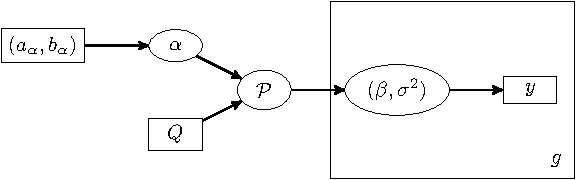
\includegraphics[width=\textwidth]{my_dag_small0}
\end{frame}

\begin{frame}[label=current]
\frametitle{DAG with augmented data}
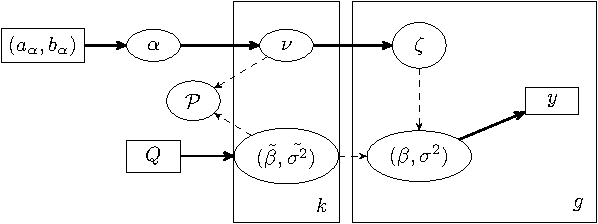
\includegraphics[width=\textwidth]{my_dag_small}
\end{frame}

\begin{frame}[label=current]
\frametitle{Full conditionals}
\begin{beamerboxesrounded}[upper=upcol,lower=lowcol,shadow=true]{Gibbs sampler}
  \begin{enumerate}
    \item Draw $\alpha$, $\zeta_g$ (conditionally independent)
    \item Draw $\pi$
    \item Draw $\tilde{\beta}_k$ (conditionally independent)
    \item Draw $\tilde{\sigma}_k$ (conditionally independent)
  \end{enumerate}
\end{beamerboxesrounded}
\end{frame}

\begin{frame}[label=current]
\frametitle{Full conditionals}
1. Draw $\alpha$, $\zeta_g$ (conditionally independent):\\

\[\alpha \sim \op{Gamma}(K + a_\alpha - 1, -\log \pi_K + b_\alpha)\]

\[\zeta_g \ind \op{Categorical}\left(\hat{\pi}_1,\ldots,\hat{\pi}_K \right),\]
with
\[\hat{\pi}_k \propto \pi_k \op{N}(y_g;X\tilde{\beta}_k,\tilde{\sigma}_k^2 W_g^{-1})\]
\end{frame}

\begin{frame}[label=current]
\frametitle{Full conditionals}
2. Draw $\pi$

\[\nu_k \ind \op{Be}(M_k + 1, \sum_{\ell>k}M_\ell + \alpha); k \le K-1,\]
where $M_k$ is the number of $\zeta_g$ equal to $k$.

Then $\pi_k = \nu_k \prod_\ell<k(1-\nu_k$.
\end{frame}

\begin{frame}[label=current]
\frametitle{Full conditionals}
3. Draw $\tilde{\beta}_k$ (conditionally independent)

\[\tilde{\beta}_k \ind \op{N}(\hat{m}_k,\, \hat{C}_k),\]
where
\[\hat{C}_k= \left( \tilde{\sigma}^{-2}_g\sum_{g:\zeta_g=k}
  X^\top W_g X + C^{-1} \right)^{-1},\]
\[\mbox{ and }\hat{m}_k=\hat{C}_k \left(\sum_{g:\zeta_g=k} X^\top W_g y_g +
      C^{-1}m \right)\]
      
\end{frame}

\begin{frame}[label=current]
\frametitle{Full conditionals}
4. Draw $\tilde{\sigma}_k^2$ (conditionally independent)

\[\tilde{\sigma}_k^2 \ind \op{IG}(\hat{a}_k,\hat{b}_k),\]
where
\[\hat{a}_k = a_{\sigma^2} + \frac{1}{2}NM_k,\mbox{ and }\]
\[\hat{b}_k= b_{\sigma^2} + \frac{1}{2}\sum_{g:\zeta_g=k}y_g^\top W_g y_g -2 \beta_g^\top X^\top W_g y_g  +\beta_g^\top X^\top W_g X \beta_g\]
\end{frame}


\begin{frame}[label=current]
\frametitle{Counts to log-cpm + precision weights}
\scalebox{.7}{
  \begin{beamerboxesrounded}[upper=upcol,lower=lowcol,shadow=true]{Definitions}
  \[r_{gn} = \mbox{count for gene }g \mbox{, sample }n;\quad g=1,\ldots,G,\quad n=1,\ldots,N\]
  \pause\[R_n = \mbox{library size for sample }n\]
  \pause\[\log \tilde{R} = \frac{1}{N}\sum_{n=1}^N \log(R_n)\]
  \pause\[y_{gn} = \log_2 \left(\frac{r_{gn}+0.5}{R_n+1}\times 10^6\right)\]
  \pause\[\tilde{r}_g = \frac{1}{N}\sum_{n=1}^N y_{gn} + \log_2(\tilde{R}) - \log_2(10^6)\]
  \pause\[s_g = \sqrt{MSE}\mbox{ from ind. OLS fits of, }y_g \sim N(X\beta_g, \sigma^2_gI_{n\timesn})\]
  \onslide<1->
  \citep{voom}  
  \end{beamerboxesrounded}
}
\end{frame}

\begin{frame}[label=current]
\frametitle{Mean-variance trend}
\only<1>{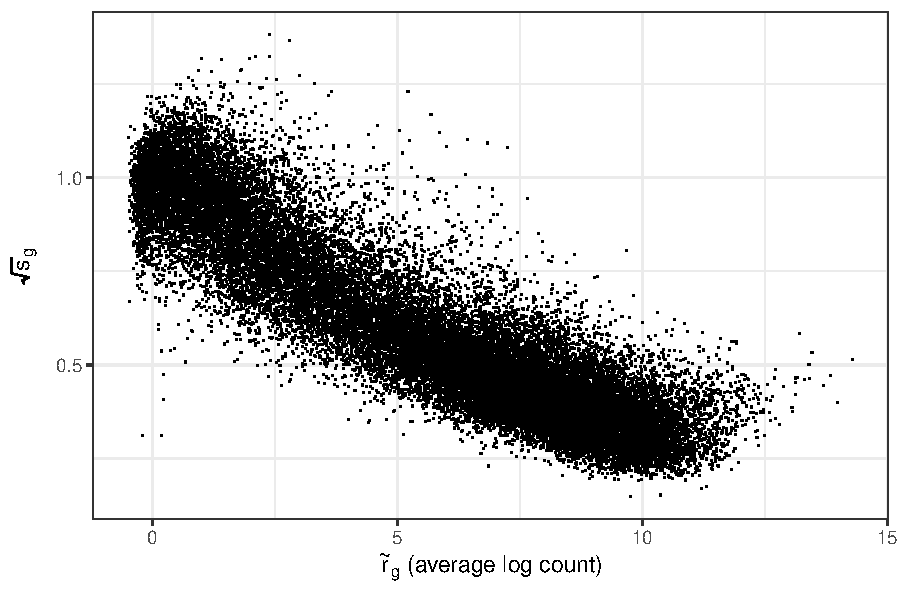
\includegraphics[width=\textwidth]{voom1}}
\only<2>{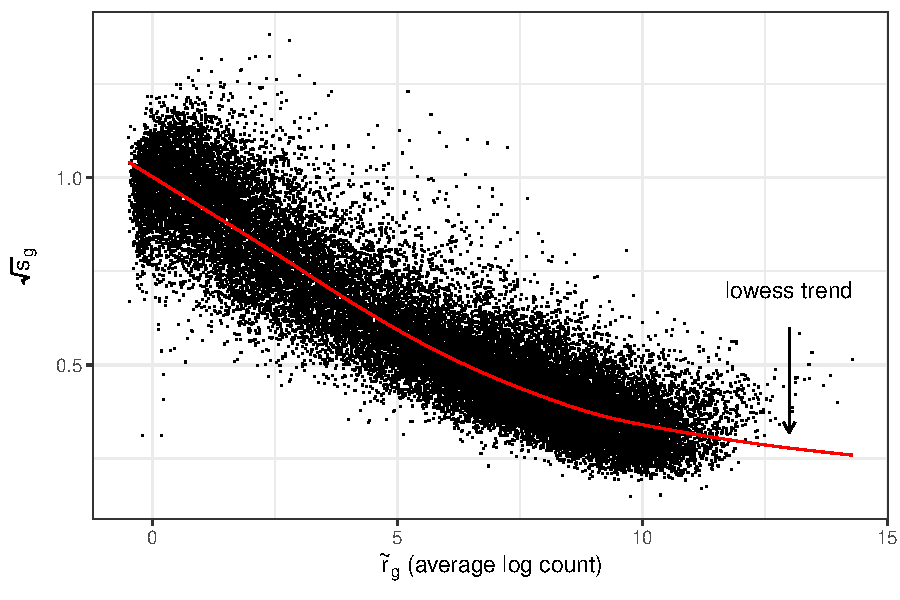
\includegraphics[width=\textwidth]{voom2}}
\end{frame}

\begin{frame}[label=current]
\frametitle{Counts to log-cpm + precision weights}
\scalebox{.6}{
  \begin{beamerboxesrounded}[upper=upcol,lower=lowcol,shadow=true]{Definitions}
  \[r_{gn} = \mbox{count for gene }g \mbox{, sample }n;\quad g=1,\ldots,G,\quad n=1,\ldots,N\]
  \[R_n = \mbox{library size for sample }n\]
  \[\log \tilde{R} = \frac{1}{N}\sum_{n=1}^N \log(R_n)\]
  \[y_{gn} = \log_2 \left(\frac{r_{gn}+0.5}{R_n+1}\times 10^6\right)\]
  \[\tilde{r}_g = \frac{1}{N}\sum_{n=1}^N y_{gn} + \log_2(\tilde{R}) - \log_2(10^6)\]
  \[s_g = \sqrt{MSE}\mbox{ from ind. OLS fits of, }y_g \sim N(X\beta_g, \sigma^2_gI_{n\timesn})\]
  \pause \[\lambda_{gn} = x_{n}\hat{\beta}_g + \log_2(R_n) - \log_2(10^6)\]
  \pause \[w_{gn} = \widehat{lowess}(\lambda_{gn})\]
  \onslide<1->
  \citep{voom}  
  \end{beamerboxesrounded}
}
\end{frame}
%%%%%%%
\section{Computation}

\begin{frame}
\frametitle{GPU computing}
\begin{itemize}
\item Scientific programming APIs have been developed for GPUs
\item GPUs offer a higher degree of parallelism with lower latency than parallel CPU computing
\item The utility of switching to GPUs is problem dependent:
\begin{itemize}
  \item The task must be broken into identical problems of similar size (preferably independent)
  \item There must be enough of these to occupy most of the GPU
  \item Typically requires more time to develop code
\end{itemize}
\end{itemize}
\end{frame}

\begin{frame}
\frametitle{Implementation overview}
I wrote an R package to wrangle RNA-seq data and perform MCMC for the BNP method. In this implementation 
\begin{itemize}
\item Parallel updates are performed on conditionally independent model parameters
\item Prerequisite computations are accelerated by the use of
\begin{itemize}
  \item Parallel reductions
  \item Parallel scans
  \item Optimized linear algebra routines, both global (large matrix multiplication) and multi-threaded (solving linear systems)
  \item Custom multi-threaded operations (ex. Cholesky decomposition)
\end{itemize}
\end{itemize}
\end{frame}

\begin{frame}
\frametitle{Example of implementation}
%\item draw_zeta
%\item weights
%\item mulinomial draw
\end{frame}

\begin{frame}
\frametitle{Running time}
\end{frame}



\section{Case study - heterosis in maize}


\begin{frame}
\frametitle{RNA-seq data}

Important features:
  
  \begin{itemize}
\item Measures associated with gene expression
\item Counts of transcripts (reads) which have been mapped to genes
\item Some variability due to sequencing process (sequencing depth, lane effects)
\item Multiple samples can be processed simultaneously
\item Typically tens of thousands of genes
\item Sample sizes tend to be limited by cost

\end{itemize}
\vspace{1cm}
{\small \citep{datta2014}}
\end{frame}

% \begin{frame}
% \frametitle{Maize RNA-seq data}
% \setkeys{Gin}{width=0.7\textwidth}

% \begin{center}
% \includegraphics{data}
% {\tiny (Will Landau)}
% \end{center}
% \end{frame}

\begin{frame}
\frametitle{Model for gene expression}
$y_{gn}$ is observed expression for gene/feature $g$, sample $n$; $y_{gn} \ge 0$.

\[\log(y_{gn}+1) \ind \op{N}\left(x_{n}^\top\beta_g, \sigma^2_g\right) \]

\begin{itemize}
\item We choose to work with a transformed version of the data for convenience

\item May be preferable to model the counts directly (later)
\end{itemize}
\end{frame}

% \begin{frame}
% \frametitle{Inferential objectives}
% We consider hypotheses of the form $H_g: c_j^\top \beta_g >0$ for all $j=1,\ldots, J$.
% \pause
% \small
% Consider the following design matrix:\\
% {\tiny
%   \[\bordermatrix{
%     & x_1 & x_2 & x_3 & x_4 \cr
%     \mbox{B73} & 1 & -1 & 0 & 0  \cr
%     \mbox{Mo17} & 1 & 1 & 0 & 0  \cr
%     \mbox{B73 x Mo17} & 1 & 0 & 1 & -1 \cr
%     \mbox{Mo17 x B73} & 1 & 0 & 1 & 1}\]
% }
% 
% \begin{itemize}
% \item $\mbox{B73} < \mbox{Mo17}$ which is simply \beta_2>0$ or $c_1^\top=\begin{pmatrix}0 & 1 & 0 & 0\end{pmatrix}$
%   
%   \item $\min \left\{ \mbox{Mo17 x B73}, \mbox{B73 x Mo17}\right\} > \max \left\{ \mbox{B73}, \mbox{Mo17} \right\}$\\
% which is simply $\min \left\{ \beta_3 + \beta_4, \beta_3 - \beta_4 \right\} > | \beta_2 |$\\
% or
% {\tiny
%   \[C^\top = \bordermatrix{
%     & & & & \cr
%     c_1 & 0 &-1 &1 &1 \cr
%     c_2 & 0 &1  &1 &1 \cr
%     c_3 & 0 &-1 &1 &-1 \cr
%     c_4 & 0 &1  &1 &-1}\]
% }
% \end{itemize}
% % Potential issues:\\
% % \begin{itemize}
% % \item Small sample size \only<2>{$\longrightarrow$ hierarchical modeling to pool information}
% % \item Multiple testing
% % \item Composite null hypotheses \only<2>{$\longrightarrow$ inferences based on joint posterior}
% % \end{itemize}
% 
% \end{frame}

% \begin{frame}{t}
% \frametitle{Data from \cite{paschold2012}}
% \begin{columns}[T]
% \begin{column}[T]{.4\textwidth}
% \begin{block}{}
% \footnotesize
% $\beta_1 = \mbox{ parental mean}$\\[.25cm]
% $\beta_2 = \mbox{ parental half-difference}$\\[.25cm]
% $\beta_3 = \mbox{ hybrid effect}$\\[.25cm]
% $\beta_4 = \mbox{ hybrid half-difference}$
%   \end{block}
% \end{column}
% 
% \begin{column}[T]{.6\textwidth}
% \resizebox{\textwidth}{!}{
%   \includegraphics{glm_pairs}
% }
% \end{column}
% \end{columns}
% \end{frame}
% 
% %%%%%%% Section 1: Introduce problem
% 
% \begin{frame}
% \frametitle{Hierarchical model}
% As a means of sharing information across genes, consider a hierarchical model,
% 
% \[(\beta_g, \sigma^2_g) \ind \mc{P}\]
% 
% \begin{itemize}
% \pause
% \item \cite{ji2014}, \cite{niemi2015empirical} proposed empirical Bayes methods; estimating $\mc{P}$ from the data and fixing $\mc{P}$ at the estimated value
% 
% \pause
% \item \cite{landau2016fully} used independent, unimodal hierarchical distributions for the components of $\beta_g$ and $\sigma^2$ and put priors on the hyperparameters
% 
% \pause
% \item \cite{liu2015semi} proposed a semiparametric model for differential expression in the case of two genotypes, used a nonparametric prior distribution for the distribution of $\rho_g$, the log-fold change for gene $g$
%   \end{itemize}
% \end{frame}
% 
% \begin{frame}
% \frametitle{Semiparametric model}
% We propose:
%   \[\mc{P} \sim \op{DP}(\alpha, Q)\]
% \pause
% Extending the approach of Liu 2015 to
% \begin{itemize}
% \item flexibly model the distribution of $\left( \beta_g,\sigma^2_g\right)$ (dependence, multimodality)
% \end{itemize}
% \pause
% While adapting the approach of Landau 2016 to
% \begin{itemize}
% \item obtain posterior estimates of \\
% $\op{Pr}(H_g|y) \approx \frac{1}{S} \sum_{s=1}^S \left[\prod_{j=1}^J 1\left(c_j^\top \beta_g^{(s)} >0 \right) \right]$
%   
%   \item maintain computational feasibility
% 
% \end{itemize}
% \end{frame}
% 
% \begin{frame}
% \frametitle{Model for gene expression}
% $y_{gn}$ is observed expression for gene/feature $g$, variety/treatment $v$, replicate $i$; $y_{gn} > 0$.
% 
% \[y_{gn} | x_{n}^\top \beta_g, \sigma^2_g \ind \op{N}\left(x_{n}^\top\beta_g, \sigma^2_g\right) \]
% \[(\beta_g, \sigma_g^2) | \mc{P} \iid \mc{P}\]
% \[\mc{P} \sim DP(\alpha, Q)\]
% \[Q=\op{N}(m, C) \times \op{IG}(a, b)\]
% 
% \end{frame}
% 
% 
% 
% % \begin{frame}
% % \frametitle{Inferential objectives}
% % Compute expectations based on $\op{p}(\beta | y)$, i.e. 
% % 
% % \[E_{\op{p}(\beta|y)}(h) = \int\;h(\beta)\;\op{p}(\beta | y) d\beta\]
% % 
% % Given MCMC samples, $\{\beta^{(i)}\}_{i=1}^{m}$, by SLLN
% % 
% % \[\op{lim}_{m\rightarrow \infty} \frac{1}{m}\sum_{i=1}^{m}h(\beta^{(i)}) \rightarrow E_{\op{p}(\beta|y)}(h)\]
% % 
% % Examples:
%   % 
% % \[h_1: \mb{R}^G \times \mb{R}^v \rightarrow \mb [0,1]^G, \quad h_1 = 1_{x_{g1}^\top \beta_g > x_{g2}^\top \beta_g} \]
% % 
% % \end{frame}
% 
% %%%%%%%% Section 2: Background
% 
% \section{Intro to DP}
% \begin{frame}
% \frametitle{Dirichlet processes}
% Definition:
%   
%   Let $(\Omega, \mathcal{F}, \mc{Q})$ be a completely separable metric space with a probability measure $\mc{Q}$ and let $\alpha > 0$. If for any finite partition of $\Omega$, $\{B_n\}_{n=1}^{N}$,
% 
% \[\mc{P}(B_1), \mc{P}(B_2), ... , \mc{P}(B_N) \sim \op{Dirichlet} \left( \alpha\mc{Q}(B_1), \alpha\mc{Q}(B_2), ..., \alpha\mc{Q}(B_N) \right),\]
% 
% then $\mc{P} \sim \op{DP}(\alpha,\mc{Q})$.
% 
% \begin{itemize}
% \item For measurable $A$, $\op{E}(\mc{P}(A)) = \mc{Q}(A),\; \op{Var}(\mc{P}(A)) = \mc{Q}(A)(1 - \mc{Q}(A))/(\alpha + 1)$
%   
%   \item $\mc{P}$ is almost surely discrete.\citep{ferguson1973}\\
% 
% \item
% For $\mc{P}_0 \ll \mc{Q}$, $\op{DP}(\alpha, \mc{Q})$ puts positive probability on distributions arbitrarily close to $\mc{P}_0$ on arbitrary sets\citep{antoniak1974}.
% \end{itemize}
% \end{frame}
% 
% 
% % \begin{frame}
% % \frametitle{Posterior Distribution}
% % 
% % \citep{ferguson1973} Let
% % 
% % \[\mc{P} \sim \op{DP}(\alpha, \mc{Q}),\]
% % 
% % \[X_1, \ldots, X_n | \mc{P} \iid \mc{P}.\]
% % 
% % Then
% % 
% % \begin{equation}\label{posterior}
% % \mc{Q}_n = \mc{P}|X_1,\ldots,X_n \sim \op{DP}(\alpha + n, \frac{\alpha}{\alpha+n}\mc{Q} + \frac{1}{\alpha+n}\sum_{i=1}^{n} \delta_{X_i})
% % \end{equation}
% % \cite{blackmac1973} proved that $\mc{Q}_n$ converges to $\mc{P}$ almost surely.
% % 
% % \end{frame}
% 
% \begin{frame}
% \frametitle{DP mixture model}
% A Dirichlet process mixture model is
% 
% \[y_g|\theta_g \ind f_{\theta_g}\]
% \[\theta_g|\mc{P} \iid \mc{P}\]
% \[\mc{P} \sim \op{DP}(\alpha,\mc{Q})\]
% 
% Here, inference for $\mc{P}$ depends on $\{S_1, S_2, \ldots, S_K\}$, where $S_k = \{g:\theta_g=\theta^*_k\}$, i.e. a random partition of the data into clusters sharing a common parameter.\\
% 
% This is a mixture model with an unknown (potentially infinite) number of components.
% 
% \end{frame}
% 
% 
% 
% 
% %%%% Paper 1
% \section{Computation}
% 
% \begin{frame}
% \frametitle{Existing software}
% \begin{itemize}
% \item {\tt DPpackage} \citep{jara2011}
% \begin{itemize}
% \item Implements (generalized) linear mixed effects models with $\op{DP}$ random effects
% \item Had problem with large data sets, unable to diagnose source of problem
% \item Has not been maintained
% \item Does not implement our model exactly
% \end{itemize}
% 
% \item {\tt Stan} Does not support discrete valued parameters
% 
% \item {\tt JAGS} Probably too slow (did not try)
% 
% \end{itemize}
% 
% \end{frame}
% 
% \begin{frame}
% \frametitle{Standard algorithms for fitting DPM model}
% A standard Gibbs sampling method targeting the posterior for the DPM model is known as the Chinese Restaurant Process (CRP)
% \[y_g|\theta, \zeta_g \ind f_{\theta_{\zeta_g}}\]
% \[\op{p}(\zeta_g|y, \alpha, \op{Q}, \zeta_{-g}) = \frac{m_k}{n + \alpha - 1}\sum_{k=1}^{K^*}\delta_k + \frac{\alpha}{n + \alpha - 1}\delta_{K^*+1}\]
% \[\theta_k \ind \op{Q}\]
% 
% where $\zeta_{-g} = \{\zeta_h: h\neq g\}$, $m_k = |\{h: \zeta_h=k\}|$ and $K^*=|\{k:\exists \zeta_h=k\}|$.
% 
% \begin{itemize}
% \item Marginalizes over the unknown $\mc{P}$
%   \item Large number of sequential Gibbs steps for $\zeta$
%   \item Potentially slow mixing
% \end{itemize}
% 
% \end{frame}
% 
% \begin{frame}
% \frametitle{Stick-breaking process}
% Let
% \begin{align}
% \label{stick}
% \begin{split}
% V_k &\iid \op{Beta}(a_k, b_k), \; k\ge 1\\
% \pi_k &= V_k \prod_{j < k}(1 - V_j); j > 1, \quad \pi_1 = V_1
% \end{split}
% \end{align}
% 
% We denote (\ref{stick}) by $\pi \sim \op{Stick}(a, b)$.
% 
% \end{frame}
% 
% \begin{frame}
% \frametitle{Stick-breaking Construction}
% \footnotesize
% 
% \cite{sethuraman1994} developed the stick-breaking construction of Dirichlet process.
% Let 
% \begin{align*}
% \theta_g &\iid \op{Q},\; i\ge 1, \; \op{Q} \text{ a probability distribution}\\
% \pi & \sim \op{Stick}(\mathbbm{1}, \alpha\mathbbm{1})
% \end{align*}
% 
% Then
% \[\mc{P} = \sum_{k=1}^{\infty} \pi_k\,\delta_{\theta_k}\]
% is a realization from $\op{DP}(\alpha,\op{Q})$.\\
% 
% An arbitrarily close approximation can be given by $\mc{P}_K \approx \mc{P}_{\infty}$, where
% \[\mc{P_{K}} = \sum_{k=1}^{K} \pi_i\,\delta_{\theta_k}.\]
% \pause
% \citep{ishwaran2000markov}
% \begin{itemize}
% \item
% Promotes rapid mixing
% \item
% approximation error decreases exponentially in $K$
%   \end{itemize}
% \end{frame}
% 
% \begin{frame}
% \frametitle{Model}
% Using the truncation approximation our model can be recast as
% \begin{align}
% \begin{split}
% y_{gvi} | x_{gv}^, \zeta_g, \beta, \sigma^2 &\ind \op{N}\left(x_{gv}^\top\beta_{\zeta_g}, \sigma^2_{\zeta_g} \right) \\
% \zeta_g|\pi &\iid \sum_{k=1}^K \pi_k\delta_k(\cdot)\\
% \pi | \alpha & \op{Stick}(1, \alpha)\\
% (\beta_k, \sigma^2_k) &\iid \op{Q}\\
% \op{Q} &= \op{N}(m, C) \times \op{IG}(a, b)
% \end{split}
% \end{align}
% \end{frame}
% 
% \begin{frame}[t]
% \frametitle{Truncated DPM model}
% \begin{columns}[T]
% \begin{column}[T]{.5\textwidth}
% Note conditional independence of:
%   \begin{itemize}
% \item $\theta_k \equiv (\beta_k, \sigma_k^2)$ given $\zeta$
%   \item $\pi$ given $\zeta$
%   \item $\zeta_g$ given $\beta, \sigma^2, \pi$
%   \end{itemize}
% \end{column}
% 
% \begin{column}[T]{.45\textwidth}
% % \resizebox{.7\textwidth}{!}{\input{tdpm.tikz}\unskip}
% \include{blockedgibbs}
% \end{column}
% \end{columns}
% \end{frame}
% 
% 
% \begin{frame}
% \frametitle{Gibbs sampler}
% \tiny
% By conditional independence,
% \begin{align*}
% p(\pi, \beta, \sigma^2 | y, \zeta) & = p(\pi | \zeta) \prod_{k=1}^{K} p( \beta ,\sigma^2| y, \zeta )\\%
% p(\zeta|y, \pi, \beta, \sigma^2) &= \prod_{g=1}^{G} p(\zeta_g|y, \pi, \beta, \sigma^2) \\
% % p(\zeta,\beta,\sigma^2,\pi|y) &\propto \left\{ \prod_{g=1}^{G} p(y_g|\beta,\sigma,\zeta)\} \cdot \\
% % & \left\{ \prod_{k=1}^K p(\beta_k,\sigma^2_k|m, C, a, b) \right\}\\
% \end{align*}
% 
% Sampling from the full conditionals can then proceed as follows:
%   \begin{align*}
% p(\pi|\zeta, \alpha) &= \op{Stick}(M + 1, T + \alpha)\\%
% p(\beta_k|y, \sigma^2_k, \zeta) &= \op{N} \left( \hat{\beta}_k, \sigma^2_k \left( \sum_{g:\zeta_g=k} X^\top X + \sigma^2_k C^{-1} \right)^{-1} \right)\\
% p(\sigma^2_k |y, \beta_k, \zeta) &= \op{IG} \left( a + M_k/2, b + \sum_{g: \zeta_g = k} (y_g - x_g^\top \beta_k )^\top ( y_g - x_g^\top \beta_k )/2 \right)\\%
% p(\zeta_g|y_g, \beta, \sigma^2, \pi) & \propto \sum_{k=1}^K \pi_k\, \op{N} (x_{gv} \beta_k, \sigma^2_k)%
% \end{align*}
% 
% $M_k:=|\{\zeta_g = k\}|$, $T_k:=|\{\zeta_g > k\}|$ and $\hat{\beta}_k$ is the posterior expectation of $\beta_k$ given $\{y_g: \zeta_g=k\}$
%   \end{frame}
% 
% \begin{frame}
% \frametitle{Using GPUs to take advantage of parallel computing capability}
% To implement our semiparametric model, we can benefit from parallelism within each iteration of our sampler
% \begin{itemize}
% \item sampling for conditionally independent parameters
% \footnote{\cite{landau2016fully} used these principles to construct a Gibbs sampler for a parametric hierarchical model using CUDA \citep{nickolls2008scalable}}
% \item reductions to compute summaries for hyperparameters \footnotemark[\value{footnote}]
% \item evaluations of the component probabilities for $\zeta$
%   \item cumulative sums to perform updates of $\pi$ as well as $\zeta$
%   \end{itemize}
% 
% \end{frame}
% 
% \begin{frame}[t,fragile]
% \frametitle{Exclusive parallel scan (cumulative sum)}
% \input{scan}
% \end{frame}
% 
% \begin{frame}
% \frametitle{Summary}
% \begin{itemize}
% \item Describe semiparametric MCMC algorithm
% 
% \item Evaluate suitability for gene expression application
% \begin{itemize}
% \item How does it scale in G?
% \item In N?
% \item Consider suitability of truncation approximation
% \end{itemize}
% \end{itemize}
% 
% \end{frame}
% 
% % \begin{frame}
% % \frametitle{Truncated approximation of DP}
% % 
% % \end{frame}
% 
% % \section{Sampling methods}
% % \begin{frame}
% % \frametitle{Review of existing methods}
% % (Blackwell and MacQueen), (Neal 2000), (Ishwaran 2001)
% % \end{frame}
% % 
% % \subsection{Polya-urn approach}
% % \begin{frame}
% % \frametitle{Polya-urn sampling}
% % A Dirichlet process $P$ drawn from $DP(\alpha)$ can be identified as the limiting distribution, updating $\mc{Q}_k$ with $\mc{Q}_{k+1} = \mc{Q}_k + \delta_{\{X_k+1\}}$, where $X_{k+1}$ is a draw from $\mc{Q}_k/\mc{Q}_k(\Omega)$ and $\mc{Q}_0 = \alpha/\alpha(\Omega)$. 
% % \end{frame}
% % 
% % \subsection{Truncated stick-breaking approach}
% % \begin{frame}
% % \frametitle{Truncated stick-breaking sampling}
% % \end{frame}
% % 
% % \section{Computational issues}
% % \begin{frame}
% % \frametitle{Computation}
% % \end{frame}
% % 
% % \subsection{DPpackage}
% % \begin{frame}
% % \frametitle{DPpackage}
% % \end{frame}
% % 
% % \subsection{Massively parallel computing}
% % \begin{frame}
% % \frametitle{Massively parallel Gibbs steps}
% % \end{frame}
% % 
% % \section{Proposed approach}
% % \begin{frame}
% % \frametitle{Proposed approach}
% % \end{frame}
% % 
% % \section{Case study: RNA-seq}
% % \begin{frame}
% % \frametitle{Case study: RNA-seq}
% % \end{frame}
% 
% \section{Case Study}
% 
% \begin{frame}
% \frametitle{Case study}
% The \cite{paschold2012} data have been analyzed by Landau \citep{landau2016fully} using a variety of parametric hierarchical models priors.
% 
% How do the results differ under a semi-parametric hierarchical model?\\
% 
% \cite{liu2015semi} proposed a Bayesian semi-parametric model for the detection of differentially expressed genes using RNA-seq data. Their model used a Poisson-Gamma mixture model for the data with a $DP$ prior on a scalar parameter, $\rho_g$ and constructed the base measure to put positive mass on null hypotheses.\\
% 
% Our model is also semiparametric, but can work with arbitrary treatment structures with more than two treatments.
% 
% \end{frame}
% 
% \begin{frame}
% \frametitle{Simulation studies}
% 
% How sensitive are our inferences to:
%   \begin{itemize}
% \item Fixing or modeling $\alpha$?
% \item Fixing or modeling $\mc{Q}$?
% \item Choice of design matrix?
% \end{itemize}
% 
% To evaluate the detection of non-null genes:
%   \begin{itemize}
% \item Simluate a series of realistic data sets as in \cite{niemi2015empirical}
% \item Fit our model and a parametric model(s) (fbseq)
% \item Rank genes by posterior probability of event of interest
% \item Compare receiver operator characteristic curves and AUC
% \end{itemize}
% \end{frame}
% 
% \section{Possible Extensions}
% 
% \begin{frame}
% \frametitle{Lognormal mixture of Poisson}
% Instead of modeling $\log(y_{gn}+1)$ as normal, it seems more natural to do as in \cite{landau2016fully}:
%   
%   \[y_{gn} \sim \op{Poisson}(\exp(X_n\,\beta_{\zeta_g} + \epsilon_{gn}))\]
% \[\epsilon_{gn} \sim N(0, \sigma^2_{\zeta_g})\]
% 
% Complications:
%   \begin{itemize}
% \item Loss of conjugacy for sampling $(\beta,\sigma^2)_k$ from full conditional
% \item Additional step to draw $\epsilon_g$
%   \end{itemize}
% \end{frame}
% 
% \begin{frame}
% \frametitle{Ge et al slice sampler}
% \footnotesize
% \cite{ge2015distributed} noted that, integrating over $\zeta_g$,
% \begin{align*}
% p(y_{g}|\theta,\pi) &= \sum_{k=1}^\infty \pi_k \, f_{\theta_k}(y_g)\\
% &= \int \sum_{k=1}^{\infty} \pi_k \, \mc{U}(u_g; 0,\pi_k)\,f_{\theta_k}(y_g)\; d\,u_g\\
% &= \int \sum_{k=1}^{\infty} \mathbbm{1}(0<u_g<\pi_k)\,f_{\theta_k}(y_g)\; d\,u_g
% \end{align*}
% 
% Conditioning on $u_g$, makes the full conditional of $\zeta_g$ depend on only finitely many terms:
%   \[p(\zeta_g| u_g, y_g, \theta, \pi) \propto \sum_{\{k:u_g<\pi_k\}} f_{\theta_k}(y_g)\]
% 
% Additionally, if we denote $K$, the number of occupied clusters, and $\pi_{K^*}$ the combined probability of all other clusters, then
% \[p(\pi_1, \pi_2, \ldots, \pi_K, \pi_{K^*}) =\op{Dirichlet}(m_1,m_2,\ldots,m_K,\alpha)\]
% \pause
% 
% \end{frame}
% 
\section[failure-time model]{A hierarchical failure-time model for observational data exhibiting infant-mortality and wearout failure modes}
% 
% \begin{frame}
% \frametitle{Data}
% (Joint work with Colin Lewis-Beck)\\
% 
% In 2013, Backblaze (\url{https://www.backblaze.com/}), a cloud storage company, began releasing daily records of its fleet of hard drives available. These hard drives continuously spin in controlled storage pods where they run until failure.  When a hard drive fails it is permanently removed, and new hard drives are continuously being added to the fleet. The data include:\\
% \begin{itemize}
% \item
% Date (yyyy-mm-dd)
% \item
% Serial Number (unit ID)
% \item
% Model (manufacturer assigned)
% \item
% Failure (indicator of last record before removed for failure)
% \item
% Hours of operation
% \item
% Capacity, and 79-89 additional SMART Stats (which we do not pay attention to)
% \end{itemize}
% \end{frame}
% 
% \begin{frame}
% \frametitle{Notation}
% \begin{itemize}
% \item $m=1,...,M$: drive model
% \item $i=1,...,n_m$: unit
% \item $y_{mi}$: number of hours a unit had operated at the end of the record
% \item $t_{mi}$: left-truncation time
% 
% \item $c_{mi}$: indicator right-censored
% \end{itemize}
% \end{frame}
% 
% \begin{frame}
% \frametitle{Model}
% \small
% The general limited failure population model \citep{chan1999failure} defines 
% \[\Phi_m = 1 - (1 - \pi\,\op{F}_{m1})\,(1 - \op{F}_{m2}),\]
% where we can choose $\op{F}_{mj}\equiv \op{F}_{\mu_{mj},\sigma_{mj}}$ be a cdf for a Weibull distribution with log-location $\mu_{mj}$, scale $\sigma_{mj}$. 
% 
% The likelihood is defined by $\prod_{m=1}^M \prod_{i=1}^{n_m} p(y_{mi}| t_{mi}, c_{mi})$ where
% \[ p(y_{mi} | t_{mi}, c_{mi}) = 
%      \begin{cases} \frac{\phi_{m}(y_{mi})}{1-\Phi_{m}(t_{mi})} & \mbox{if } c_{mi} = 0\\
%    \frac{1-\Phi_{m}(y_{mi})}{1 - \Phi_{m}(t_{mi})} & \mbox{if } c_{mi}=1
%    \end{cases}\]
% Further, we model
% {\tiny
%   \[ (\log(q_{p_1,m1}), \log(\sigma_{m1}), \log(q_{p_2,m2}), \log(\sigma_{m2}), \op{logit}(\pi_{m}))^\top \ind \op{N}(\eta, \op{diag}(\tau)\,I),\]
% }
% where $q_{p_j,mj}$ is the $p_j^{th}$ quantile of $\op{F}_{mj}$. (This re-parameterization improves numerical stability because of the heavy right censoring.)
% \end{frame}
% 
% \begin{frame}
% \frametitle{Failure distribution estimation}
% \includegraphics[height=.8\textheight]{overview_dm_compare}
% 
% \tiny Weibull plots with pointwise posterior 95\% credible intervals and Kaplan-Meier estimate for 22 drive models.
% \end{frame}
% 
% \begin{frame}
% \frametitle{Results}
% \begin{itemize}
% \item Approach allows flexible modeling of failure distributions for heterogenous systems with mostly censored/incomplete data
% \item Hierarchical modeling provides automatic, data-dependent regularization of parameters
% \item Working implementation using off-the-shelf software
% \end{itemize}
% \end{frame}
% 

\begin{frame}[allowframebreaks]
\tiny
\frametitle{References}
\bibliographystyle{agsm}
\bibliography{../mybib}

\end{frame}

\begin{frame}[label=current]
\frametitle{Acknowledgment}
\small%
This research was supported by National Institute of General Medical Sciences (NIGMS) of the National Institutes of Health and the joint National Science Foundation / NIGMS Mathematical Biology Program under award number R01GM109458. The content is solely the responsibility of the authors and does not necessarily represent the official views of the National Institutes of Health or the National Science Foundation.
\end{frame}

\end{document}